\begin{frame}{Introducción al procesamiento de señal}
	\begin{block}{\centering \footnotesize Digitalización}
		%\centering
		Proceso mediante el cual, una señal analógica $x_a(t)$ continua en tiempo y valores pasa a una señal digital $x_d(t)$ discreta en tiempo y valores.
	\end{block}
	\begin{figure}[ht!]
		\centering
		\resizebox{\textwidth}{!}{
			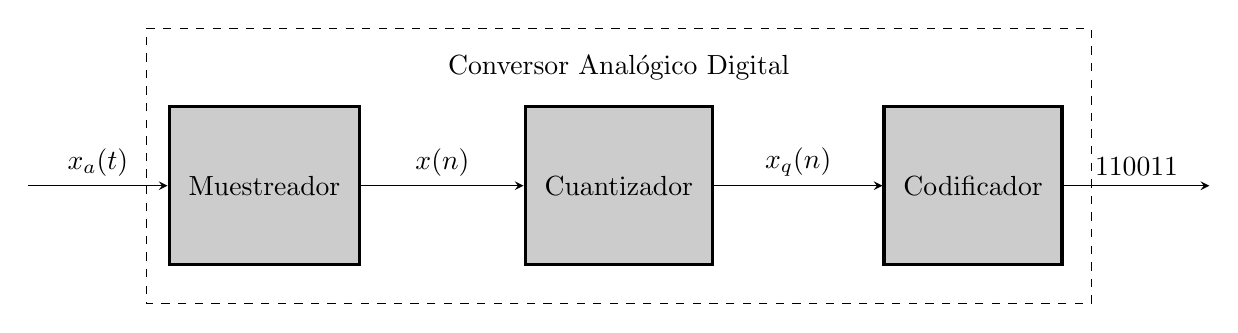
\begin{tikzpicture}
			\tikzstyle{box} = [draw,inner sep=7,minimum size=57,line 
			width=1, very thick, draw=black, fill=black!20]
			\tikzstyle{invisible} = [outer sep=0,inner sep=0,minimum size=0]
			\tikzstyle{stealth} = [-stealth]
			\node [box] (v1) at (-1,0.5) {Muestreador};
			\node [box] (v2) at (3.5,0.5) {Cuantizador};
			\node [box] (v3) at (8,0.5) {Codificador};
			\draw [stealth] (v1) edge node [anchor=south] {$x(n)$} (v2);
			\draw [stealth] (v2) edge node [anchor=south] {$x_q(n)$} (v3);
			\node [invisible] (v4) at (-4,0.5) {};
			\draw [stealth] (v4) edge node [anchor=south] {$x_a(t)$} (v1);
			\node [invisible] (v5) at (11,0.5) {};
			\draw [stealth] (v3) edge node [anchor=south] {$110011$} (v5);
			\draw [dashed] (-2.5,2.5) node [invisible] (v6) {} -- (9.5,2.5) node [invisible] {} -- 
			(9.5,-1) node [invisible] {} -- (-2.5,-1) node [invisible] {} -- (v6);
			\node [invisible] at (3.5,2) {Conversor Analógico Digital};
			\end{tikzpicture}
		}      
		\caption{Esquema de la conversión analógico a digital}
	\end{figure}
\end{frame}
\begin{frame}{Introducción al procesamiento de señal. Muestreo I}
	\begin{block}{\centering \footnotesize Digitalización}
		%\centering
		Proceso mediante el cual, una señal analógica $x_a(t)$ continua en tiempo y valores pasa a una señal $x(n)$ discreta en tiempo y continua en valores.
	\end{block}
	\begin{figure}[ht!]
		\centering
		\resizebox{0.6\textwidth}{!}{
			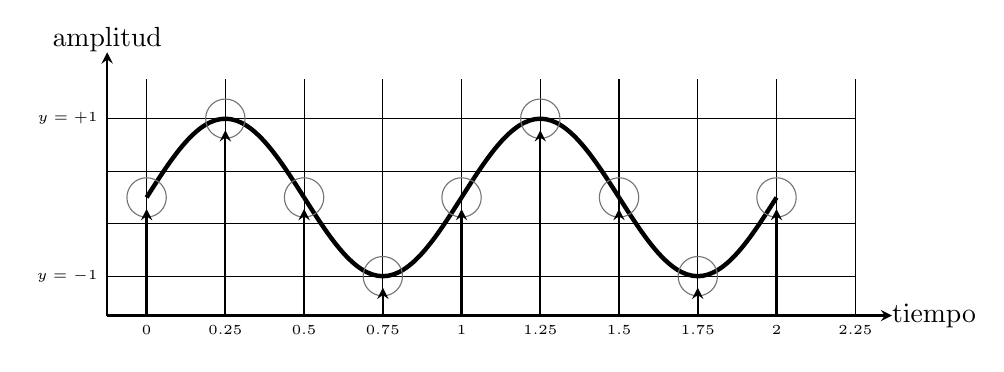
\begin{tikzpicture}
			\tikzstyle{stealth} = [-stealth, thick]
			\tikzstyle{invisible} = [outer sep=0,inner sep=0,minimum size=0]
			\tikzstyle{circle} = [shape=circle, minimum size=0.5cm, draw=black!55]
			\draw (-0.5,1)node[left,font=\tiny] {$y=+1$} -- (9,1);
			\draw (-0.5,-1)node[left,font=\tiny] {$y=-1$} -- (9,-1);
			\draw (-0.5,-0.33)node[left,font=\tiny] {} -- (9,-0.33); 
			\draw (-0.5,0.33)node[left,font=\tiny] {} -- (9,0.33); 
			\foreach \x in {0,0.25,...,2.25}
			{
				\draw (\x*4,-1.5)node [below,font=\tiny,] {\x } -- (\x*4,1.5) ;
			}
			\draw[ultra thick, ] (0,0) node (v5) {} sin (1,1) node (v7) {};
			\draw[ultra thick, ] (1,1) cos (2,0) node (v9) {};
			\draw[ultra thick, ] (2,0) sin (3,-1) node (v11) {};
			\draw[ultra thick, ] (3,-1) cos (4,0) node (v13) {};
			\draw[ultra thick, ] (4,0)  sin (5,1) node (v15) {};
			\draw[ultra thick, ] (5,1) cos (6,0) node (v17) {};
			\draw[ultra thick, ] (6,0) sin (7,-1) node (v19) {};
			\draw[ultra thick, ] (7,-1) cos (8,0) node (v21) {}; 
			\node [invisible] (v1) at (-0.5,-1.5) {};
			\node [invisible] (v2) at (-0.5,2) {amplitud};
			\node [invisible] (v3) at (10,-1.5) {tiempo};
			\draw [stealth] (v1) edge (v2);
			\draw [stealth] (v1) edge (v3);
			\node [circle] at (0,0) {};
			\node [circle] at (1,1) {};
			\node [circle] at (2,0) {};
			\node [circle] at (3,-1) {};
			\node [circle] at (4,0) {};
			\node [circle] at (5,1) {};
			\node [circle] at (6,0) {};
			\node [circle] at (7,-1) {};
			\node [circle] at (8,0) {};
			\node [invisible] (v4) at (0,-1.5) {};
			\node [invisible] (v6) at (1,-1.5) {};
			\node [invisible] (v8) at (2,-1.5) {};
			\node [invisible] (v10) at (3,-1.5) {};
			\node [invisible] (v12) at (4,-1.5) {};
			\node [invisible] (v14) at (5,-1.5) {};
			\node [invisible] (v16) at (6,-1.5) {};
			\node [invisible] (v18) at (7,-1.5) {};
			\node [invisible] (v20) at (8,-1.5) {};
			\draw [stealth] (v4) edge (v5);
			\draw [stealth] (v6) edge (v7);
			\draw [stealth] (v8) edge (v9);
			\draw [stealth] (v10) edge (v11);
			\draw [stealth] (v12) edge (v13);
			\draw [stealth] (v14) edge (v15);
			\draw [stealth] (v16) edge (v17);
			\draw [stealth] (v18) edge (v19);
			\draw [stealth] (v20) edge (v21);
			\end{tikzpicture}
		}      
		\caption{Esquema del muestreo de una señal de 1Hz muestreada a 4 muestras por segundo}
		\label{fig: sample}
	\end{figure}
\end{frame}
\begin{frame}{Introducción al procesamiento de señal. Muestreo II}
	\begin{block}{\centering \footnotesize Teorema de muestreo de Nyquist-Shannon}
		Si la frecuencia más alta contenida en una señal analógica $x_{a}(t)$ es $F_{max}=B$ y la señal se muestrea a una tasa $F_{s}>2F_{max}\equiv 2B$, entonces $x_{a}(t)$ se puede recuperar totalmente a partir de sus muestras mediante la siguiente función de interpolación
		\begin{align}
		g(t)&=\frac{\sin 2\pi Bt}{2\pi Bt} \\ \nonumber
		&\text{Así, }x_{a}(t)\text{ se puede expresar como:} \\ \nonumber
		x_{a}(t)&=\sum _{n=-\infty }^{\infty }x_{a}\left({\frac {n}{F_{s}}}\right)g\left(t-{\frac {n}{F_{s}}}\right)\\ \nonumber
		&\text{donde }x_{a}\left({\frac {n}{F_{s}}}\right)=x_{a}\left(nT\right)\equiv x\left(n\right)\text{ son las muestras de }x_{a}\left(t\right)
		\end{align}
	\end{block}
	\vspace*{-10pt}
	\begin{columns}
		\column[]{0.45\textwidth}
		{
			\begin{figure}[ht!]
				\centering
				\resizebox{0.8\textwidth}{!}{
					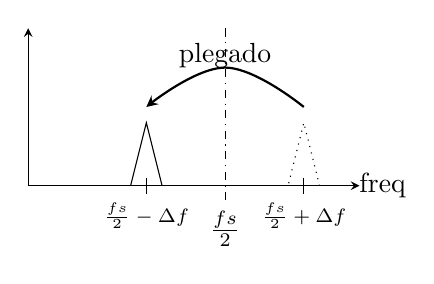
\begin{tikzpicture}
					\tikzstyle{invisible} = [outer sep=0,inner sep=0,minimum size=0]
					\tikzstyle{stealth} = [-stealth]
					\node [invisible] (v1) at (0,0) {};
					\node [invisible] (v2) at (0,2) {};
					\node [invisible] (v3) at (4.5,0) {freq};
					\draw [stealth] (v1) edge (v2);
					\draw [stealth] (v1) edge (v3);
					\draw [dashdotted](2.5,2) -- (2.5,-0.2) node[anchor=north]{$\frac{fs}{2}$};
					
					\draw [invisible, dotted](3.7,0) node [circle] {} -- 
					(3.5,0.8) node [circle] {} -- 
					(3.3,0) node [circle] {};
					\draw [draw](3.5,0.1) -- (3.5,-0.1) node[anchor=north]{\scriptsize$\frac{fs}{2} + \Delta f$};
					\draw [invisible](1.7,0) node [circle] {} -- 
					(1.5,0.8) node [circle] {} -- 
					(1.3,0) node [circle] {};
					\draw [draw](1.5,0.1) -- (1.5,-0.1) node[anchor=north]{\scriptsize$\frac{fs}{2} - \Delta f$};
					\draw [invisible, thick, stealth] plot[smooth, tension=.7] coordinates {(3.5,1) (2.5,1.5) (1.5,1)};
					\node [invisible, anchor=south] at (2.5,1.5) {plegado};
					\end{tikzpicture}
				}
				\vspace*{-10pt}
				\caption{Esquema del plegado de una señal con aliasing}
				\label{fig: aliasing_mirror}
			\end{figure}
		}
		\column[]{0.45\textwidth}
		{
			\begin{figure}
				\centering
				\begin{subfigure}[t]{0.5\textwidth}
					\centering
					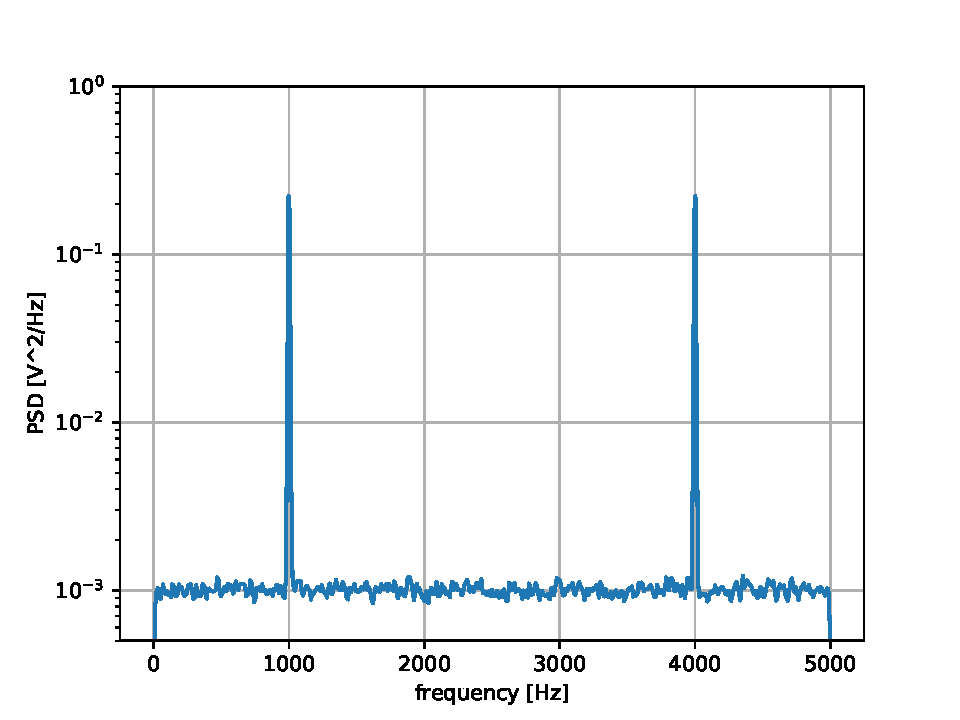
\includegraphics[width=0.9\textwidth]{../figures/pwelch_1k_4k_10k}
					\vspace*{-5pt}
					\caption{Densidad espectral de potencia para la suma dos senos de 1kHz y 4kHz muestreados a 10ksps}
				\end{subfigure}%
				\hspace*{10pt}
				\begin{subfigure}[t]{0.5\textwidth}
					\centering
					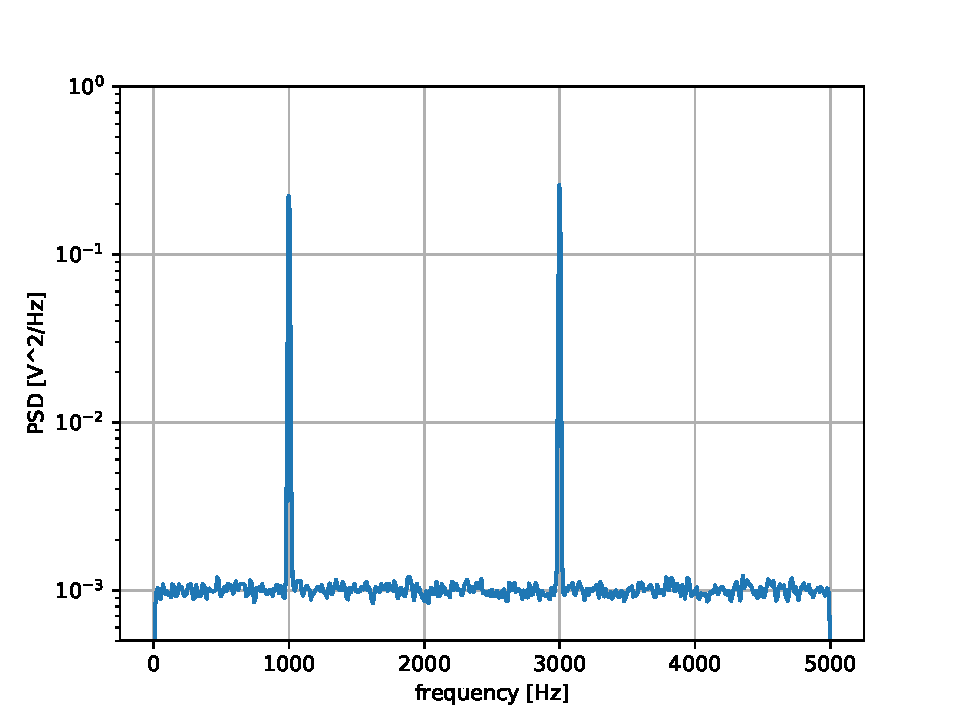
\includegraphics[width=0.9\textwidth]{../figures/pwelch_1k_7k_10k}
					\vspace*{-5pt}
					\caption{Densidad espectral de potencia para la suma dos senos de 1kHz y 7kHz submuestreados a 10ksps}
				\end{subfigure}
				\label{fig: aliasing}
			\end{figure}
		}
	\end{columns}
\end{frame}
\begin{frame}{Introducción al procesamiento de señal. Cuantización}
	\begin{block}{\centering \footnotesize Digitalización}
		%\centering
		Proceso mediante el cual, una señal $x(n)$ discreta en tiempo y continua en valores pasa a una señal digital $x_q(n)$ discreta en tiempo y en valores.
	\end{block}
	\begin{columns}
		\column[]{0.45\textwidth}
		{
			\begin{figure}[ht!]
				\centering
				\resizebox{\textwidth}{!}{
					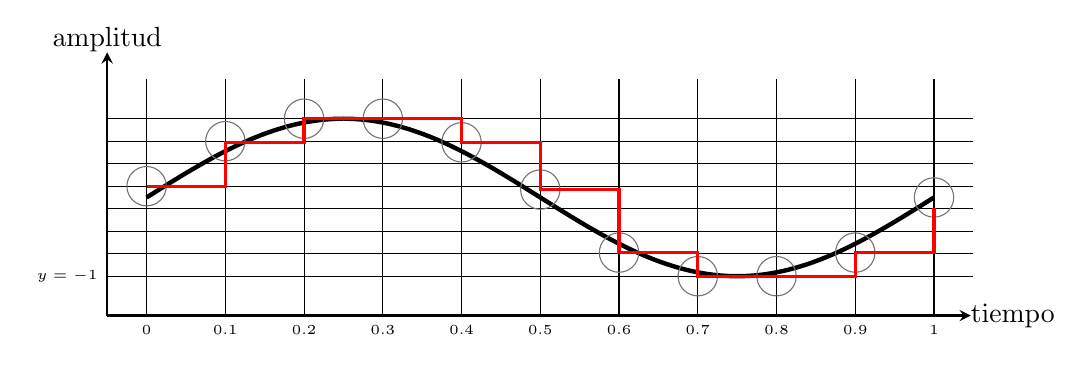
\begin{tikzpicture}
					\tikzstyle{stealth} = [-stealth, thick]
					\tikzstyle{invisible} = [outer sep=0,inner sep=0,minimum size=0]
					\tikzstyle{circle} = [shape=circle, minimum size=0.5cm, draw=black!55]
					\tikzstyle{line} = [draw, very thick, red]
					\draw (-0.5,1)node[left,font=\tiny] {} -- (10.5,1);
					\draw (-0.5,0.7142)node[left,font=\tiny] {} -- (10.5,0.7142);
					\draw (-0.5,0.4285)node[left,font=\tiny] {} -- (10.5,0.4285);
					\draw (-0.5,0.1428)node[left,font=\tiny] {} -- (10.5,0.1428);
					\draw (-0.5,-0.1428)node[left,font=\tiny] {} -- (10.5,-0.1428);
					\draw (-0.5,-0.4285)node[left,font=\tiny] {} -- (10.5,-0.4285);
					\draw (-0.5,-0.7142)node[left,font=\tiny] {} -- (10.5,-0.7142);
					\draw (-0.5,-1)node[left,font=\tiny] {$y=-1$} -- (10.5,-1);
					\foreach \x in {0,0.1,0.2,0.3,0.4,0.5,0.6,0.7,0.8,0.9,1}
					{
						\draw (\x*10,-1.5)node [below,font=\tiny,] {\x } -- (\x*10,1.5) ;
					}
					\draw[ultra thick, ] (0,0) node (v5) {} sin (2.5,1) node (v7) {};
					\draw[ultra thick, ] (2.5,1) cos (5,0) node (v9) {};
					\draw[ultra thick, ] (5,0) sin (7.5,-1) node (v11) {};
					\draw[ultra thick, ] (7.5,-1) cos (10,0) node (v13) {};
					
					\node [invisible] (v1) at (-0.5,-1.5) {};
					\node [invisible] (v2) at (-0.5,2) {amplitud};
					\node [invisible] (v3) at (11,-1.5) {tiempo};
					\draw [stealth] (v1) edge (v2);
					\draw [stealth] (v1) edge (v3);
					\node [circle] (v4) at (0,0.1428) {};
					\node [circle] (v6) at (1,0.7142) {};
					\node [circle] (v8) at (2,1) {};
					\node [circle] (v10) at (3,1) {};
					\node [circle] (v12) at (4,0.7) {};
					\node [circle] (v14) at (5,0.1) {};
					\node [circle] at (6,-0.7) {};
					\node [circle] (v15) at (7,-1) {};
					\node [circle] at (8,-1) {};
					\node [circle] (v16) at (9,-0.7) {};
					\node [circle] (v17) at (10,0) {};
					\draw [line](0,0.1428) -- (1,0.1428) node [invisible] {} -- (1,0.7) -- 
					(2,0.7) node [invisible] {} -- (2,1) -- 
					(4,1) node [invisible] {} -- (4,0.7) -- 
					(5,0.7) node [invisible] {} -- (5,0.1) node [invisible] {} --
					(6,0.1) -- (6,-0.7) node [invisible] {} --
					(7,-0.7) node [invisible] {} -- (7,-1) -- 
					(9,-1) node [invisible] {} -- (9,-0.7) -- (10,-0.7) -- (10,-0.14);
					\end{tikzpicture}
				}      
				\caption{Esquema de la cuantización con 4 bits a 10 muestras por segundo, i.e., 8 valores posibles}
				\label{fig: cuantization_4bit}
			\end{figure}
		}
		\column[]{0.45\textwidth}
		{
			\begin{figure}[ht!]
				\centering
				\resizebox{\textwidth}{!}{
					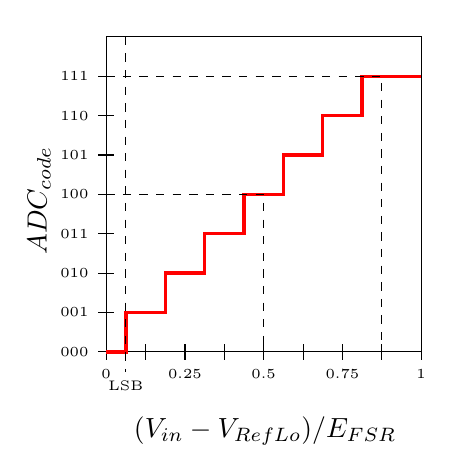
\begin{tikzpicture}
					\tikzstyle{stealth} = [-stealth, thick]
					\tikzstyle{invisible} = [outer sep=0,inner sep=0,minimum size=0]
					\tikzstyle{circle} = [shape=circle, minimum size=0.5cm, draw=black!55]
					\tikzstyle{line} = [draw, very thick, red]
					
					\draw (0,0) node [invisible] (v1) {} --
					(4,0) node [invisible] {} --
					(4,4) node [invisible] {} --
					(0,4) node [invisible] {} --
					(0,0) node [invisible] {};
					\foreach \x in {0,0.25,0.5,0.75,1}
					{
						\draw (\x*4,-0.1)node [below,font=\tiny,] {\x } -- (\x*4,0.1) ;
					}
					\foreach \x in {0.125,0.375,0.625,0.875,1}
					{
						\draw (\x*4,-0.1)node [below,font=\tiny,] {} -- (\x*4,0.1);
					}
					\foreach \c [count=\x from 0] in {{000},{001},{010},{011},{100},{101},{110},{111}}
					{
						\draw (-0.1,\x*0.5)node [anchor=east,font=\tiny,] {\c} -- (0.1,\x*0.5);
					}
					%\node at (0,\x) {\c};	
					\draw [line](v1) -- (0.25,0) node [invisible] {} -- 
					(0.25,0.5) node [invisible] {} -- 
					(0.75,0.5) node [invisible] {} -- 
					(0.75,1) node [invisible] {} -- 
					(1.25,1) node [invisible] {} -- 
					(1.25,1.5) node [invisible] {} -- 
					(1.75,1.5) node [invisible] {} -- 
					(1.75,2) node [invisible] {} -- 
					(2.25,2) node [invisible] {} -- 
					(2.25,2.5) node [invisible] {} -- 
					(2.75,2.5) node [invisible] {} -- 
					(2.75,3) node [invisible] {} -- 
					(3.25,3) node [invisible] {} -- 
					(3.25,3.5) node [invisible] {} -- 
					(4,3.5) node [invisible] {};
					\node [invisible] at (2.0187,-1) {$(V_{in}-V_{RefLo})/E_{FSR}$};
					\node [invisible, rotate=90] at (-0.8509,1.9232) {$ADC_{code}$};
					\draw [dashed](0,2) node [invisible] {} -- (2,2) node [invisible] {} -- (2,0) node [invisible] {};
					\draw [dashed](0,3.5) node [invisible] {} -- (3.5,3.5) node [invisible] {} -- (3.5,0) node [invisible] {};
					\draw [dashed](0.25,4) node [] {} -- (0.25,-0.25) node [anchor=north] {\tiny LSB};
					\end{tikzpicture}
				}      
				\caption{Resolución del ADC}
				\label{fig: adc_resolution}
			\end{figure}
		}
	\end{columns}
\end{frame}